\documentclass[11pt]{article}

\usepackage{geometry}
\usepackage{graphicx}
\usepackage{siunitx}
\usepackage{amsmath}
\usepackage{amssymb}
\usepackage{enumerate}
\usepackage{multirow}
\usepackage{indentfirst}
\usepackage{float}

\geometry{top=1.3in, bottom=1.3in, left=1.0in, right=1.0in}

\setlength{\parindent}{2em}

\newcommand{\e}[1]{\times10^{#1}}
\newcommand{\degree}{^\circ}

\linespread{1.3}

\begin{document}

\begin{titlepage}

\newcommand{\HRule}{\rule{\linewidth}{0.5mm}}

\center

\textsc{\LARGE UM - SJTU Joint Institute}\\[1cm]
\textsc{\Large Physics Laboratory I}\\[0.5cm]
\textsc{\large VP141}\\[0.5cm]

\HRule \\[0.4cm]
{
    \bfseries
    {\huge Exercise II}\\[0.3cm]
    {\large Measurement of Fluid Viscosity}\\[0.2cm]
    \HRule \\[1.5cm]
}

\begin{minipage}{0.6\textwidth}

\large
\emph{Name:}\\
Tianyi \textsc{Ge} \\

\emph{Student Number:}\\
516370910168 \\

\emph{Group:}\\
17\\

\emph{Instructor:}\\
Prof. Mateusz \textsc{Krzyzosiak}

\end{minipage}\\[3.5cm]

{\large \today}\\[2cm]

\vfill

\end{titlepage}
\section{Introduction}
    The objectives of this exercise include measuring the moment of inertia of a rigid body with the constant-torque method. The dependence of the moment of inertia on mass distribution and on the choice of the rotation axis will be studied. The parallel axis (Steiner's) theorem can be verified. This exercise also involves the operation of a photo-gate electronic timer.

    Moment of inertia of a rigid body about an axis characterizes the body's resistance (inertia) to change of angular velocity in rotation about that axis. It's determined by both its mass and mass distribution. If the rigid body obtains an irregular shape or non-uniformly distributed mass, we can easily use experimental methods to calculate it.

\subsection{Second law of dynamics for rotational motion}
    The second law of dynamics for rotational motion about a fixed axis is 
    \begin{equation}
        \tau_z=I\beta_z,
    \end{equation}
    relates the component of the torque $tau_z$ about the axis of rotation with the moment of inertia about this axis, and the angular acceleration component $\beta_c$. Therefore, the moment of inertia $I$ can be found with these two quantities measured.

    Also we know that the moment of inertia is additive. The moment of inertia of a combined rigid body $AB$ composed of $A$ and $B$, about the same axis of rotation, is
    \[
        I_{AB}=I_A+I_B.
    \]

\subsection{Parallel axis theorem}
    If the moment of inertia of a rigid body about the axis through the body's center of mass is $I_0$, the nfor any axis parallel to that, the moment of inertia is
    \begin{equation}
        I=I_0+md^2,
    \end{equation}
    where $d$ is the distance between the two axes. This theorem is known as Parallel axis theorem or Steiner's theorem.
\section{Experimental Setup}
    The measurement equipment consists of the following elements: springs, Jolly balance, air track, electronic timer, electronic balance and masses.\\
    \begin{figure}[h]
        \centering
        \begin{minipage}{0.4\linewidth}
            A: Sliding bar with metric scale;\\
            H: Vernier for reading;\\
            C: Small mirror with a horizontal line in the middle;\\
            D: Fixed glass tube also with a horizontal line in the middle;\\
            G: Knob for ascending and descending the sliding bar;\\
            S: Spring attached to top of the bar A.\\
        \end{minipage}
        \hspace{0.8cm}
        \begin{minipage}{0.35\linewidth}
            \label{jolly}
            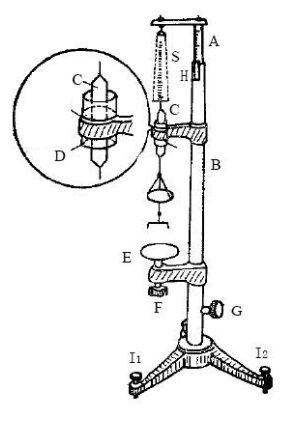
\includegraphics[height=6cm]{images/2.png}
        \end{minipage}
        \caption{Jolly balance}
    \end{figure}

    In order to measure the spring constant using the Jolly balance, we need to place the small mirror $C$ (see Figure \ref{jolly}) in the tube $D$ and make three lines coincide: the line on the mirror, the line on the glass tube and its reflection in the mirror. First, without adding any weight on the bottom end of the spring, adjust the knob G and make the three lines coincide. Then read the scale $L_1$.
    
    Second, add mass m to the bottom of the spring. The spring is stretched and the three lines no longer coincide. Adjust knob G to make them into one line again and read the corresponding number on scale $L_2$. The spring constant may be then found as
    \begin{equation}
        k=\frac{mg}{L_2-L_1}
    \end{equation}
    so that we can estimate the spring constant by finding a linear fit to the data using the least squares method.\\

    \begin{figure}[h]
        \centering
        \label{airtrack}
        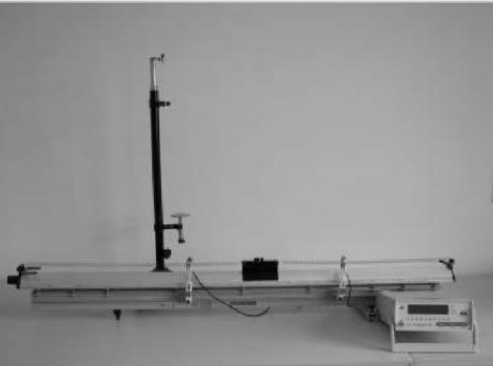
\includegraphics[height=6.5cm]{images/3.png}
        \caption{The experimental setup}
    \end{figure}

    A photoelectric measuring system consists of two photoelectric gates and an electronic timer. When a shutter on the object blocks the light, the computer will record the time. For period measurements, we use the I-shape shutter.

    When measuring the instaneous speed, the U-shape shutter is required. $\Delta t$ presents the time interval when the object travels a distance of $\Delta x=(x_{in}+x_{out})/2$. Hence we estimate the speed as $v=\Delta x/\Delta t$.

    \begin{figure}[h]
        \centering
        \label{U}
        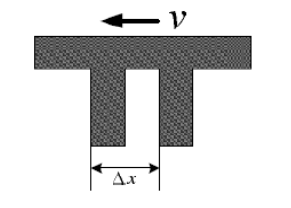
\includegraphics[height=3cm]{images/4.png}
        \caption{The U-shape shutter}
    \end{figure}
\section{Measurement Procedure}
\begin{enumerate}
    \item Measure the mass of the weight, the hoop, the disk and the cylinder, as well as the radius of the cone pulley and the cylinder (following the instructor's requirements). Calculate the moment of inertia of the hoop and the disk analytically.\\
    Use a reliable source to find the local value of the acceleration due to gravity in Shanghai.
    \item Turn the electronic timer on and switch it to mode 1-2 (single gate, multiple pulses).
    \item Place the instrument close to the edge of the desk and stretch the disk pulley arm outside so that the weight can move downwards unobstructed.
    \item Level the turntable with bubble level.
    \item Make the turntable rotating and press the start button on the timer. After at least 8 signals are recorded, stop the turntable and record the data in your data sheet.
    \item Attach the weight to one end of the string. Place the string on the disk pulley, thread through the hole in the arm, and wind the string around the third ring of the cone pulley. Adjust the arm holder so that the string goes through the center of the hole.
    \item Release the weight and the start the timer. Stop the turntable when the weight hits the floor. Write down the recorded data.
    \item The angular acceleration can be found by plotting $\theta=k\pi$ against $t$ and performing a quadratic fit using data processing software. (The magnitude of the angular acceleration is equal to the coefficient next to $t^2$ multiplied by two. The uncertainty of the angular acceleration can be read directly from the fitting result.)
\end{enumerate}
\section{Results}
\subsection{Measurements for spring constant}
    From the raw spring length measurement data in Table \ref{spring}, we obtain the change amount of the spring length by $\Delta_{L_i}=L_i-L_0$ in Table \ref{spring*}.

    Since the acceleration due to gravity is exactly $9.794m/s^2$, we obtain the weights of weight stacks from their masses, as shown in Table \ref{weight}.
    \begin{table}[htbp]
        \centering
        \begin{tabular}{|c|c|c|c|c|c|}
            \hline
            \multicolumn{6}{|c|}{Unit: $[\times 10^{-2}m]\pm 0.01[\times 10^{-2}m]$}\\ \hline
            No. & spring 1 & No. & spring 2 & No. & series\\ \hline
            $L_0$ & 2.25 & $L_0$ & 2.84 & $L_0$ & 5.06\\ \hline
            $L_1$ & 4.40 & $L_1$ & 4.96	& $L_1$ & 9.25\\ \hline
            $L_2$ & 6.56 & $L_2$ & 7.08 & $L_2$ & 13.38\\ \hline
            $L_3$ & 8.70 & $L_3$ & 9.18	& $L_3$ & 17.60\\ \hline
            $L_4$ & 10.78 & $L_4$ & 11.25 & $L_4$ & 21.98\\ \hline
            $L_5$ & 12.85 & $L_5$ & 13.30 & $L_5$ & 26.09\\ \hline
            $L_6$ & 15.03 & $L_6$ &	15.42 & $L_6$ &	30.31\\ \hline
        \end{tabular}
        \caption{Spring constant measurement data}\label{spring}
    \end{table}
    \begin{table}[htbp]
        \centering
        \begin{tabular}{|c|c|c|c|c|c|}
            \hline
            \multicolumn{6}{|c|}{Unit: $[\times 10^{-2}m]\pm 0.01[\times 10^{-2}m]$}\\ \hline
            No. & spring 1 & No. & spring 2 & No. & series\\ \hline
            $\Delta_{L_1}$ & 2.15 & $\Delta_{L_1}$ & 2.12 & $\Delta_{L_1}$ & 4.19\\ \hline
            $\Delta_{L_2}$ & 4.31 & $\Delta_{L_2}$ & 4.24 & $\Delta_{L_2}$ & 8.32\\ \hline
            $\Delta_{L_3}$ & 6.45 & $\Delta_{L_3}$ & 6.34 & $\Delta_{L_3}$ & 12.54\\ \hline
            $\Delta_{L_4}$ & 8.53 & $\Delta_{L_4}$ & 8.41 & $\Delta_{L_4}$ & 16.92\\ \hline
            $\Delta_{L_5}$ & 10.60 & $\Delta_{L_5}$ & 10.46 & $\Delta_{L_5}$ & 21.03\\ \hline
            $\Delta_{L_6}$ & 12.78 & $\Delta_{L_6}$ & 12.58 & $\Delta_{L_6}$ & 25.25\\ \hline
        \end{tabular}
        \caption{Calculated spring measurement data}\label{spring*}
    \end{table}
    \begin{table}[htbp]
        \centering
        \begin{tabular}{|c|c|c|}
            \hline
            & $m[\times 10^{-3}kg]\pm 0.01[\times 10^{-3}kg]$ & $W[\times 10^{-3}N]\pm 0.1[\times 10^{-3}N]$\\ \hline
            1 & 4.83 & 47.3\\ \hline
            2 & 9.65 & 94.5\\ \hline
            3 & 14.50 & 142.0\\ \hline
            4 & 19.24 & 188.4\\ \hline
            5 & 23.99 & 235.0\\ \hline
            6 & 28.80 & 282.1\\ \hline            
        \end{tabular}
        \caption{Weight measurement data}\label{weight}
    \end{table}
    The relation between the elastic force and the change of spring length is linear.Using the least-squares method, we can calculate the most optimal estimate of the slope and intercept. The errorbars of $W$ and $\Delta_L$ are based on their own combined uncertainties, which is just their type $B$ uncertainties $\Delta_B$ in this case. Specific error calculaton is included in section 5.

    The errorbar is \textbf{not clear enough} because the error is relatively \textbf{small}. The sample calculation of $k_1$ done by Matlab is also shown here. The fitting curve in Figure \ref{k_1} is based on Table \ref{k1data}.
    \begin{table}
        \centering
        \begin{tabular}{|c|c|c|c|c|}
            \hline
            No. & $\Delta_L[m]$ & $u_{\Delta_L}[m]$ & $W[N]$ & $u_{W}[N]$\\ \hline
            1 & 0.0215 & 0.0001 & 0.04730 & 0.0001\\ \hline
            1 & 0.0431 & 0.0001 & 0.09451 & 0.0001\\ \hline
            1 & 0.0645 & 0.0001 & 0.1420 & 0.0001\\ \hline
            1 & 0.0853 & 0.0001 & 0.1884 & 0.0001\\ \hline
            1 & 0.1060 & 0.0001 & 0.2350 & 0.0001\\ \hline
            1 & 0.1278 & 0.0001 & 0.2821 & 0.0001\\ \hline
        \end{tabular}
        \caption{Data for $W vs. \Delta_L$ of spring 1 in Figure \ref{k_1}}\label{k1data}
    \end{table}
    \begin{figure}[h]    
        \begin{minipage}{0.5\linewidth}
            \[
            \begin{split}
                k_1&=\frac{\overline{\Delta_LW}-\overline{\Delta_L}\cdot\overline{W}}{\overline{\Delta_L^2}-\overline{\Delta_L}^2}\\[0.2cm]
                &\approx \frac{1.52\times10^{-2}-7.47\times10^{-2}\times0.165}{68.9\times10^{-4}-55.8\times10^{-4}}\\[0.2cm]
                &=2.22\pm 0.02kg/s^2.\\[0.4cm]
                u_{r,k_1}&=0.9\%
                %b_1&=\overline{W}-k_1\overline{\Delta_L}\\[0.2cm]
                %&\approx 0.1649\times 2.22 \times 0.07470\\[0.2cm]
                %&=(-6.25\pm 12.5)\times10^{-4}N.
            \end{split}
            \]
        \end{minipage}
        \begin{minipage}{0.4\linewidth}
            \centering
            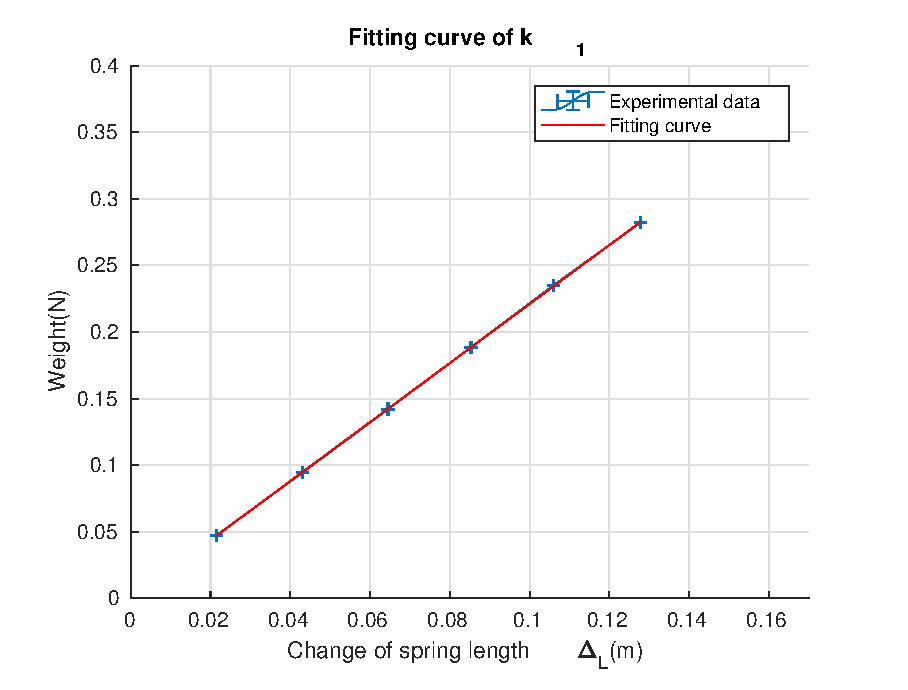
\includegraphics[height=6.7cm]{images/k1.eps}
            \caption{Fitting curve of spring 1}\label{k_1}
        \end{minipage}
    \end{figure}
    \newpage
    \begin{figure}[!h]
        \centering
        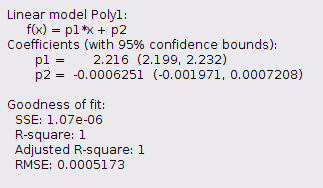
\includegraphics[height=5.8cm]{images/k1info.png}
        \caption{Information of fit in Figure \ref{k_1}}\label{k1info}
    \end{figure}
    Simliarly, we obtain $k_2$ and $k_3$.
    \begin{table}[!htbp] \small
        \centering
        \begin{tabular}{|c|c|c|c|c|}
            \hline
            No. & $\Delta_L[m]$ & $u_{\Delta_L}[m]$ & $W[N]$ & $u_{W}[N]$\\ \hline
            1 & 0.0212 & 0.0001 & 0.04730 & 0.0001\\ \hline
            1 & 0.0424 & 0.0001 & 0.09451 & 0.0001\\ \hline
            1 & 0.0634 & 0.0001 & 0.1420 & 0.0001\\ \hline
            1 & 0.0841 & 0.0001 & 0.1884 & 0.0001\\ \hline
            1 & 0.1046 & 0.0001 & 0.2350 & 0.0001\\ \hline
            1 & 0.1258 & 0.0001 & 0.2821 & 0.0001\\ \hline
        \end{tabular}
        \caption{Data for $W vs. \Delta_L$ of spring 2 in Figure \ref{k_2}}\label{k2data}
    \end{table}
    \begin{figure}[!h]
        \centering
        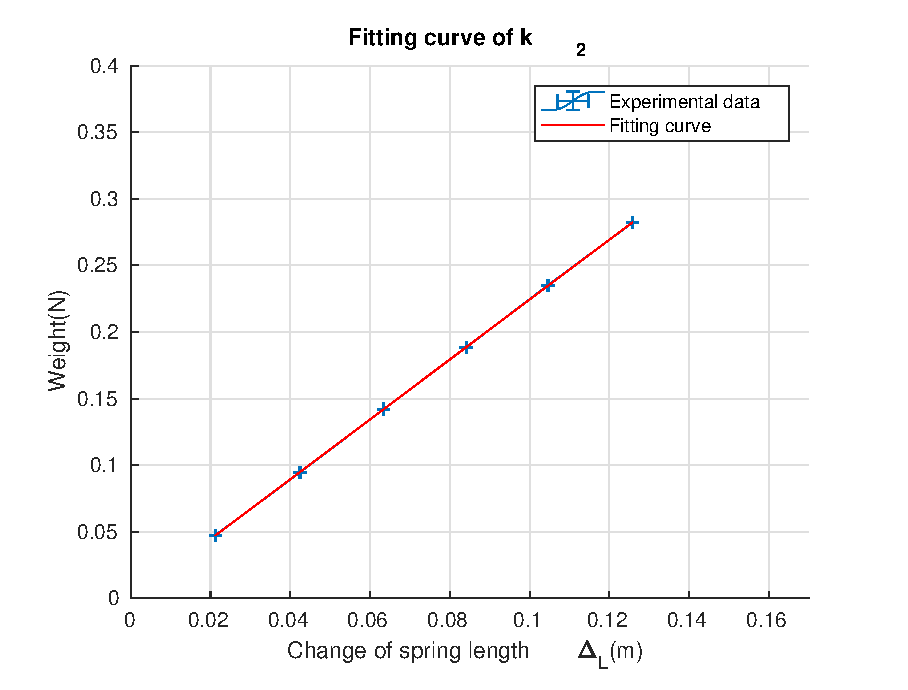
\includegraphics[height=6cm]{images/k2.eps}
        \caption{Fitting curve of spring 2}\label{k_2}
    \end{figure}
    \begin{figure}[!h]
        \centering
        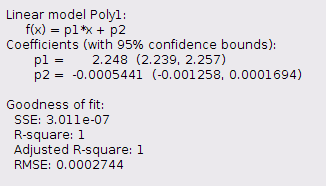
\includegraphics[height=5cm]{images/k2info.png}
        \caption{Information of fit in Figure \ref{k_2}}\label{k2info}
    \end{figure}
    \[
        k_2\approx 2.25\pm 0.01kg/s^2, \quad u_{r,k_2}=0.4\%
        %b_2&\approx (-5.44\pm 70) \times10^{-4}N.
    \]
    \begin{table}[!ht] \small
        \centering
        \begin{tabular}{|c|c|c|c|c|}
            \hline
            No. & $\Delta_L[m]$ & $u_{\Delta_L}[m]$ & $W[N]$ & $u_{W}[N]$\\ \hline
            1 & 0.0419 & 0.0001 & 0.04730 & 0.0001\\ \hline
            2 & 0.0832 & 0.0001 & 0.09451 & 0.0001\\ \hline
            3 & 0.1254 & 0.0001 & 0.1420 & 0.0001\\ \hline
            4 & 0.1692 & 0.0001 & 0.1884 & 0.0001\\ \hline
            5 & 0.2103 & 0.0001 & 0.2350 & 0.0001\\ \hline
            6 & 0.2525 & 0.0001 & 0.2821 & 0.0001\\ \hline
        \end{tabular}
        \caption{Data for $W vs. \Delta_L$ of spring series in Figure \ref{k_3}}\label{k3data}
    \end{table}
    \newpage
    \begin{figure}[h]
        \centering    
        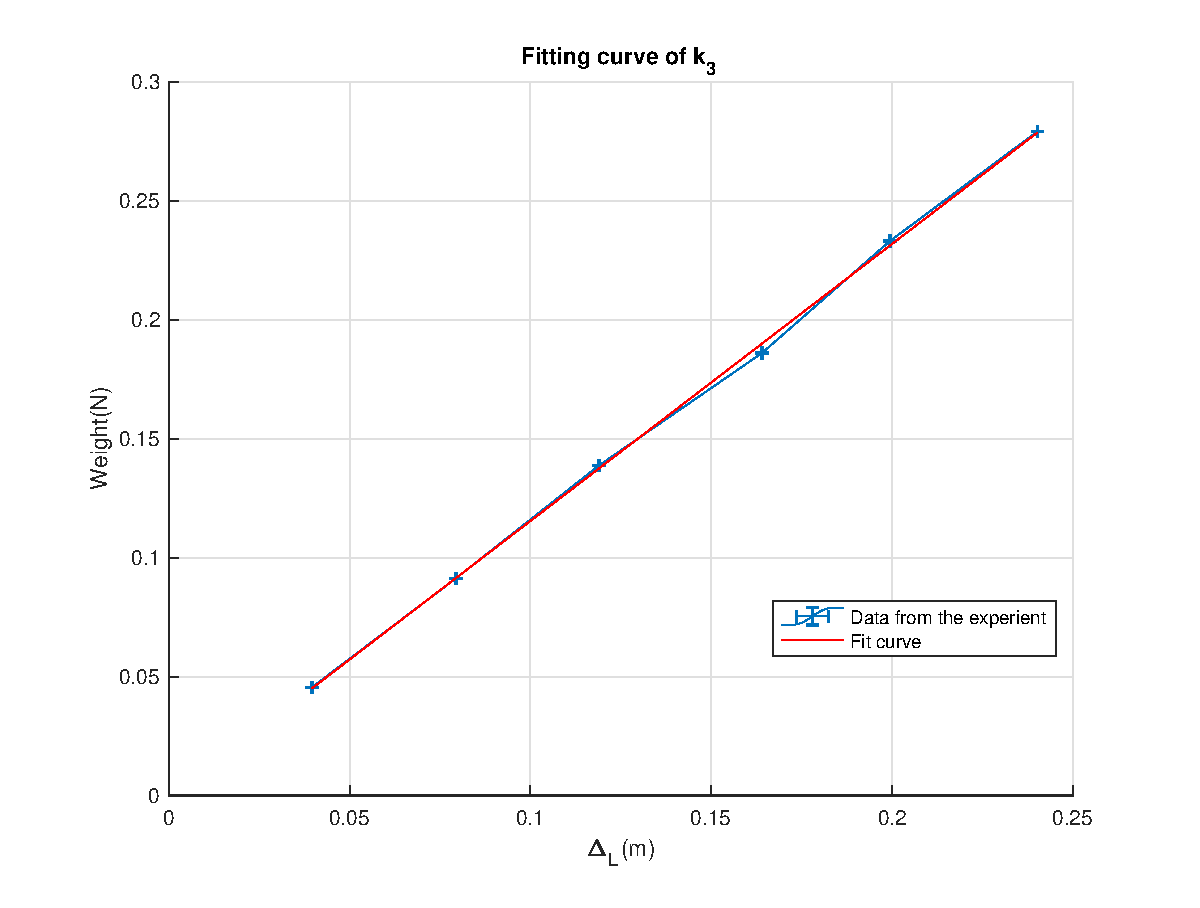
\includegraphics[height=7cm]{images/k3.eps}
        \caption{Fitting curve of series of spring 1 and spring 2}\label{k_3}
    \end{figure}
    \begin{figure}[!h]
        \centering
        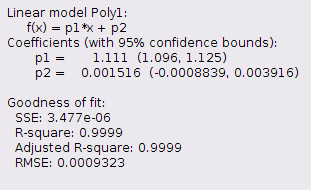
\includegraphics[height=5cm]{images/k3info.png}
        \caption{Information of fit in Figure \ref{k_3}}\label{k3info}
    \end{figure}
    \[
        k_3\approx 1.11\pm 0.017kg/s^2, \quad u_{r,k_3}=1.5\%
        %b_3&\approx (15.1\pm 20)\times10^{-4}N.
    \]

    However, $k_3$ could be theoretically calculated by $k_1$ and $k_2$. This will be further discussed in Section 5.\\

\subsection{Relation between the period $T$ and the mass $M$}
    In this experiment we use I-shape shutter to block the photoelectric gate. The mass data are listed in Table \ref{M} and. The effective mass in Table \ref{M} is the sum of $m_{objI}$ and the mass of weights in Table \ref{weight}.

    \begin{table}[h]
        \centering
        \begin{tabular}{|c|c|}
            \hline
            object with I-shape & $m_{objI}=176.55\pm 0.01[\times10^{-3}kg]$\\ \hline
            object with U-shape & $m_{objU}=186.75\pm 0.01[\times10^{-3}kg]$\\ \hline
            mass of spring 1 & $m_{spr1}=10.74\pm 0.01[\times10^{-3}kg]$\\ \hline
            mass of spring 2 & $m_{spr2}=10.77\pm 0.01[\times10^{-3}kg]$\\ \hline
            equivalent mass & $M_I=m_{objI}+\frac{1}{3}m_{spr1}+\frac{1}{3}m_{spr2}=183.72\pm 0.01[\times10^{-3}kg]$\\ \hline
            equivalent mass & $M_U=m_{objU}+\frac{1}{3}m_{spr1}+\frac{1}{3}m_{spr2}=193.92\pm 0.01[\times10^{-3}kg]$\\ \hline
        \end{tabular}
        \caption{Mass measurement data}\label{M}
    \end{table}
    \vspace{1cm}
    %\begin{table}[h]
    %    \centering
    %    \begin{tabular}{|c|c|c|c|c|c|c|}
    %        \hline
    %        \multicolumn{6}{|c|}{Ten periods $[\times10^{-3}s]\pm0.1[\times10^{-3}s]$} & Effective mass\\ \hline
    %        \multicolumn{2}{|c|}{horizontal} & \multicolumn{2}{|c|}{incline 1} & \multicolumn{2}{|c|}{incline 2} & $[\times10^{-3}]\pm 0.01[\times10^{-3}kg]$\\ \hline
    %        $m_1$ & 12798.9 & $m_1$ & 12804.1 & $m_1$ & 12800.1 & 188.55\\ \hline
    %        $m_1$ & 12964.9 & $m_2$ & 12957.0 & $m_2$ & 12955.4 & 193.37\\ \hline
    %        $m_1$ & 13127.2 & $m_3$ & 13123.7 & $m_3$ & 13127.0 & 198.22\\ \hline
    %        $m_1$ & 13282.6 & $m_4$ & 13282.7 & $m_4$ & 13275.6 & 202.96\\ \hline
    %        $m_1$ & 13436.3 & $m_5$ & 13439.3 & $m_5$ & 13436.3 & 207.71\\ \hline
    %        $m_1$ & 13592.4 & $m_6$ & 13591.6 & $m_6$ & 13594.9 & 212.52\\ \hline
    %    \end{tabular}
    %    \caption{Measurement data for the T vs. M relation}\label{T}
    %\end{table}
    Again using the least-squares method we can plot the fitting curve of $T^2 vs. M$ (see Figure \ref{tm}). The errorbar is still not clear though.

    \begin{table}[h] \small
        \centering
        \begin{tabular}{|c|c|c|c|c|}
            \hline
            No. & $M[kg]$ & $u_{M}[kg]$ & $T^2[s^2]$ & $u_{T^2}[s^2]$\\ \hline
            1 & 0.18855 & 0.000015 & 1.63812 & 0.00003\\ \hline
            2 & 0.19337 & 0.000015 & 1.68089 & 0.00003\\ \hline
            3 & 0.19822 & 0.000015 & 1.72323 & 0.00003\\ \hline
            4 & 0.20296 & 0.000015 & 1.76427 & 0.00003\\ \hline
            5 & 0.20771 & 0.000015 & 1.80534 & 0.00003\\ \hline
            6 & 0.21252 & 0.000015 & 1.84753 & 0.00003\\ \hline
        \end{tabular}
        \caption{Data for $T^2 vs. M$ for the horizontal track in Figure \ref{tm}}\label{tmdata}
    \end{table}
    \begin{figure}[!h]
        \centering    
        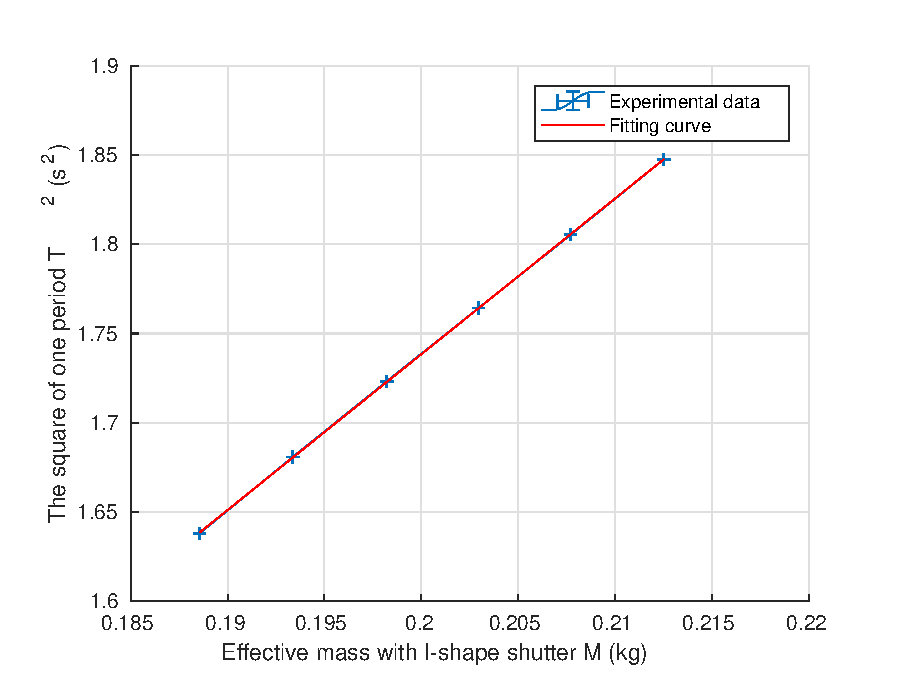
\includegraphics[height=9cm]{images/tm.eps}     
        \caption{$T^2 vs. M$ for the horizontal track.$\quad slope_{hor}=8.72\pm 0.05s^2/kg,\quad u_{r,hor}=0.6\%.$}\label{tm}
    \end{figure}
    \begin{figure}[!h]
        \centering
        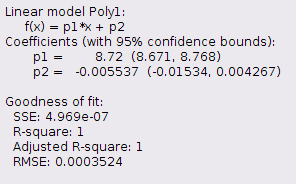
\includegraphics[height=5cm]{images/tminfo.png}
        \caption{Information of fit in Figure \ref{tm}}\label{tminfo}
    \end{figure}
    \begin{table}
        \centering
        \begin{tabular}{|c|c|c|c|c|}
            \hline
            No. & $M[kg]$ & $u_{M}[kg]$ & $T^2[s^2]$ & $u_{T^2}[s^2]$\\ \hline
            1 & 0.18855 & 0.000015 & 1.63945 & 0.00003\\ \hline
            2 & 0.19337 & 0.000015 & 1.67884 & 0.00003\\ \hline
            3 & 0.19822 & 0.000015 & 1.72232 & 0.00003\\ \hline
            4 & 0.20296 & 0.000015 & 1.76430 & 0.00003\\ \hline
            5 & 0.20771 & 0.000015 & 1.80615 & 0.00003\\ \hline
            6 & 0.21252 & 0.000015 & 1.84732 & 0.00003\\ \hline
        \end{tabular}
        \caption{Data for $T^2 vs. M$ for incline 1 in Figure \ref{tmi1}}\label{tmi1data}
    \end{table}
    \begin{figure}[!h]
        \centering
        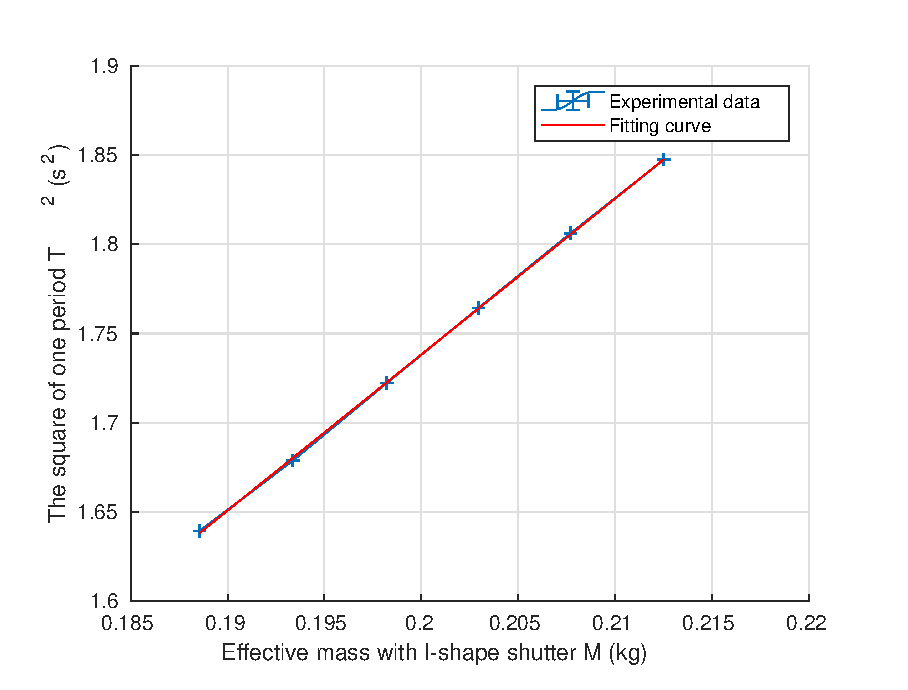
\includegraphics[height=6cm]{images/tmi1.eps}
        \caption{$T^2 vs. M$ for incline 1. $\quad slope_{inc1}=8.73\pm 0.14s^2/kg,\quad u_{r,inc1}=1.6\%.$}\label{tmi1}
    \end{figure}
    \begin{figure}[!h]
        \centering
        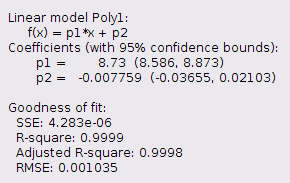
\includegraphics[height=5cm]{images/tmi1info.png}
        \caption{Information of fit in Figure \ref{tmi1}}\label{tmi1info}
    \end{figure}
    \begin{table}\small
        \centering
        \begin{tabular}{|c|c|c|c|c|}
            \hline
            No. & $M[kg]$ & $u_{M}[kg]$ & $T^2[s^2]$ & $u_{T^2}[s^2]$\\ \hline
            1 & 0.18855 & 0.000015 & 1.63843 & 0.00003\\ \hline
            2 & 0.19337 & 0.000015 & 1.67842 & 0.00003\\ \hline
            3 & 0.19822 & 0.000015 & 1.72318 & 0.00003\\ \hline
            4 & 0.20296 & 0.000015 & 1.76242 & 0.00003\\ \hline
            5 & 0.20771 & 0.000015 & 1.80534 & 0.00003\\ \hline
            6 & 0.21252 & 0.000015 & 1.84821 & 0.00003\\ \hline
        \end{tabular}
        \caption{Data for $T^2 vs. M$ for incline 2 in Figure \ref{tmi2}}\label{tmi2data}
    \end{table}

    \begin{figure}[!h]
        \centering
        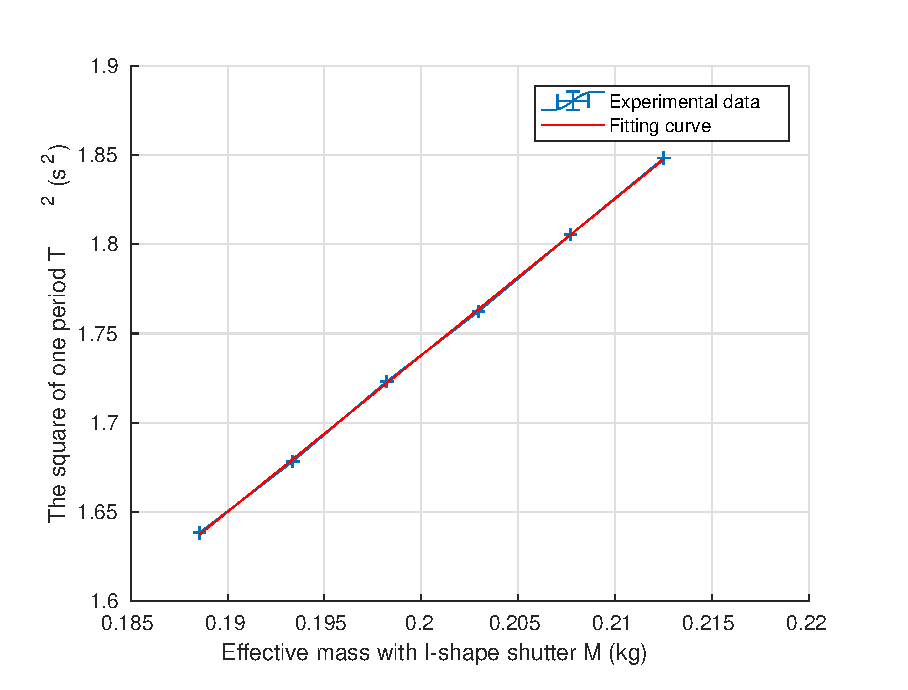
\includegraphics[height=8cm]{images/tmi2.eps}
        \caption{$T^2 vs. M$ for incline 2. $\quad slope_{inc2}=8.76\pm 0.17s^2/kg,\quad u_{r,inc2}=1.9\%.$}\label{tmi2}
    \end{figure}
    \begin{figure}[h]
        \centering
        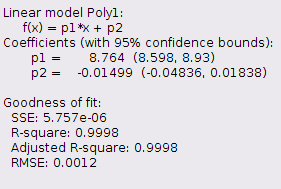
\includegraphics[height=5cm]{images/tmi2info.png}
        \caption{Information of fit in Figure \ref{tmi2}}\label{tmi2info}
    \end{figure}
    From the results above, we can conclude that therelation between $T^2$ and $M$ is that $T^2\propto M$. Whether it's incline or horizontal will not affect the relation. 

\subsection{Relation between period $T$ and amplitude $A$}
    \begin{table}[h] \small
        \centering
        \begin{tabular}{|c|c|c|c|c|}
            \hline
            No. & $A[m]$ & $u_{A}[m]$ & $T[s]$ & $u_{T}[s]$\\ \hline
            1 & 0.05 & 0.001 & 1.26451 & 0.0001\\ \hline
            2 & 0.10 & 0.001 & 1.26361 & 0.0001\\ \hline
            3 & 0.15 & 0.001 & 1.26287 & 0.0001\\ \hline
            4 & 0.20 & 0.001 & 1.26358 & 0.0001\\ \hline
            5 & 0.25 & 0.001 & 1.26362 & 0.0001\\ \hline
            6 & 0.30 & 0.001 & 1.26360 & 0.0001\\ \hline
        \end{tabular}
        \caption{Data for $A\ vs.\ T$ in Figure \ref{at}}\label{atdata}
    \end{table}
    \begin{figure}[!h]
        \centering
        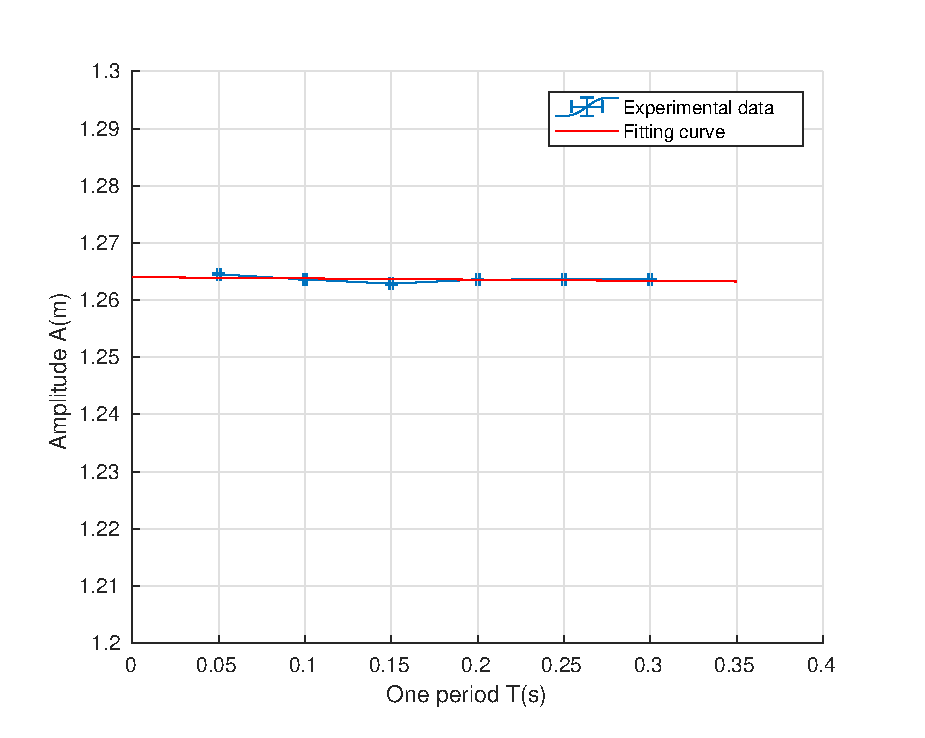
\includegraphics[height=7cm]{images/at.eps}
        \caption{Fitting curve of $T\ vs.\ A$, $\quad slope=(-2.18\pm7)\times10^{-3}s/m, \quad u_r=300\%$}\label{at}
    \end{figure}
    \vspace{0.6cm}
    \begin{figure}[h]
        \centering
        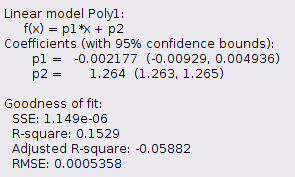
\includegraphics[height=5cm]{images/atinfo.png}
        \caption{Information of fit in Figure \ref{at}}\label{atinfo}
    \end{figure}
    To figure out whether $T$ depends on A, we need to calculate the correlation coefficient $\gamma$. The results generated by Matlab shows that
    \[
        \gamma_{A,T}=\frac{cov(A,T)}{s_A\cdot s_T}=\frac{\sum(A-\bar{A})(T-\bar{T})}{ns_A\cdot s_T}\approx -0.391.
    \]
    In fact we know that the period $T$ is independent on $A$, which means the theoretical value of $\gamma$ should be $0$. Nevertheless, the experimental value shows that $T$ and $A$ is weakly correlated. This will be discussed in section 6.

\subsection{Relation between the maximum speed and the amplitude}
    First, we need the average values of $x_{in}$ and $x_{out}$ using the data from Table \ref{x}.
    \begin{table}[h] \small
        \centering
        \begin{tabular}{|c|c|c|}
            \hline
            No. & $x_{in}[\times10^{-3}m]\pm 0.02[\times10^{-3}m]$ & $x_{out}[\times10^{-3}m]\pm 0.02[\times10^{-3}m]$\\ \hline
            1 & 4.48 & 15.40\\ \hline
            2 & 4.52 & 15.40\\ \hline
            3 & 4.46 & 15.42\\ \hline
        \end{tabular}
        \caption{Data for the calculation of $\Delta x$}\label{x}
    \end{table}
    \[
    \begin{split}
        x_{in}&=\frac{1}{3}\sum_{i=1}^{3}x_{in,i}=\frac{0.00448+0.00452+0.00446}{3}\\
        &=(4.49\pm0.08)\times10^{-3}m,\quad u_{r,x_{in}}=1.8\%.\\[0.4cm]
        x_{out}&=\frac{1}{3}\sum_{i=1}^{3}x_{out,i}=\frac{0.01540+0.01540+0.01542}{3}\\
        &=(15.41\pm0.03)\times10^{-3}m,\quad u_{r,x_{out}}=0.2\%.\\
    \end{split}
    \]
    \[
    \begin{split}
        \Delta x&=(x_{in}+x_{out})/2\\
        &=(9.95\pm0.04)\times10^{-3}m,\quad u_{r,\Delta x}=0.4\%.
    \end{split}
    \]

    \begin{table}[h] \small
        \centering
        \begin{tabular}{|c|c|c|c|c|}
            \hline
            No. & $A^2[m^2]$ & $u_{A^2}[m^2]$ & $v_{max}^2[m^2/s^2]$ & $u_{v_{max}^2}[m^2/s^2]$\\ \hline
            1 & 0.0025 & 0.0001 & 0.0570 & 0.0005\\ \hline
            2 & 0.0100 & 0.0002 & 0.233 & 0.002  \\ \hline
            3 & 0.0225 & 0.0003 & 0.518 & 0.004  \\ \hline
            4 & 0.0400 & 0.0004 & 0.907 & 0.007  \\ \hline
            5 & 0.0625 & 0.0005 & 1.41 & 0.012   \\ \hline
            6 & 0.0900 & 0.0006 & 2.00 & 0.017   \\ \hline
        \end{tabular}
        \caption{Data for the fitting curve in Figure \ref{va}}\label{vadata}
    \end{table}
    \begin{figure}[!h]
        \centering
        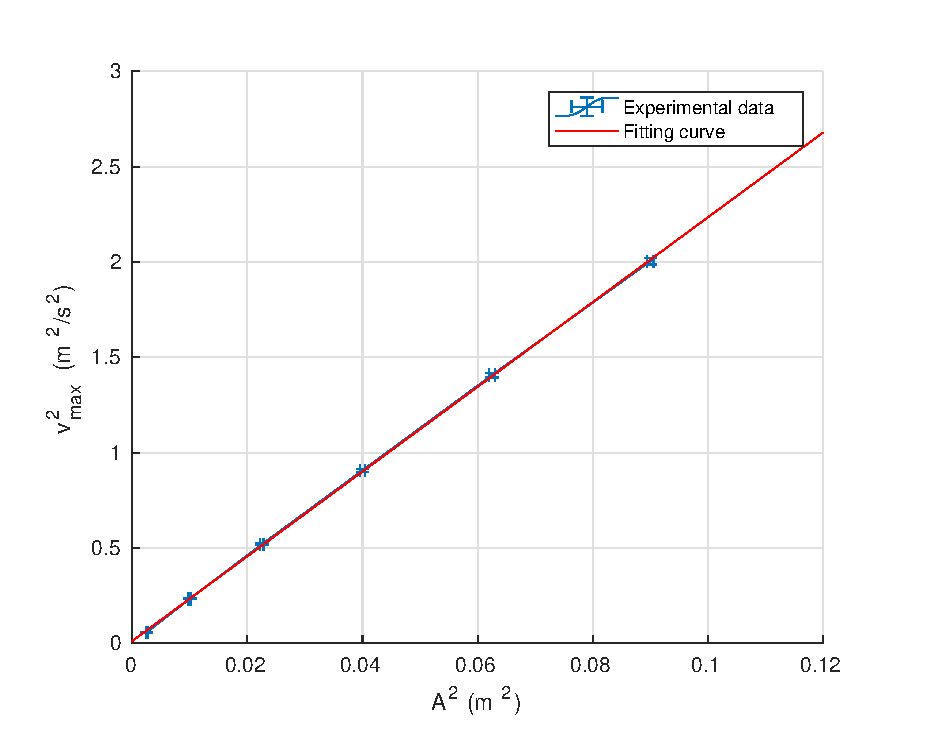
\includegraphics[height=6cm]{images/va.eps}
        \caption{Fitting curve of $v_{max}^2\ vs.\ A^2$, $\quad slope=22.22\pm0.31s^{-2}, \quad u_r=1.4\%$}\label{va}
    \end{figure}
    \begin{figure}[!h]
        \centering
        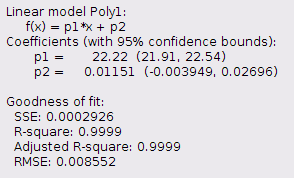
\includegraphics[height=5cm]{images/vainfo.png}
        \caption{Information of fit in Figure \ref{va}}\label{vainfo}
    \end{figure}
\section{Measurement Uncertainty Analysis}
\subsection{Uncertainty of spring constants}
    To determine the uncertainty of $\Delta L=L_i-L_0$, we need that
    \[
    \begin{split}
        &\frac{\partial \Delta L}{\partial L_i}=1,\quad \frac{\partial \Delta L}{\partial L_0}=-1,\\
        &u_{L_i}=u_{L_0}=\Delta_{dev}=1\times10^{-4}m,\\
        &u_{\Delta L}=\sqrt{(\frac{\partial \Delta L}{\partial L_i})^2\cdot (u_{L_i})^2+(\frac{\partial \Delta L}{\partial L_0})^2\cdot (u_{L_0})^2}=\sqrt{2}\times 1\times10^{-4}\approx1.4\times10^{-4}m.\\
    \end{split}
    \].
    Similarly, $u_{W}$ of $W=mg$ is
    \[
    \begin{split}
        \frac{\partial W}{\partial m}&=g=9.794kg\cdot m/s^2,\\
        u_m&=\Delta_{dev}=1\times10^{-5}kg,\\
        u_{W}&=\sqrt{(\frac{\partial W}{\partial m})^2\cdot (u_m)^2}=\sqrt{(9.794)^2\times (1\times10^{-5})^2}\approx 0.1\times10^{-3}N.\\
    \end{split}
    \].
    The error of $\Delta L$ and $W$ will be shown in errorbar.
\subsubsection{Uncertainty of fitting spring constants}
    The standard deviation of least-squares method is calculated by
    \[
        \sigma_W=\sqrt{\frac{1}{k-n}\sum_{i=1}^{k}\varepsilon_i^2},
    \]
    where $k$ is the number of measurements and $n$ is the number of unknown quantity. In this experiment, we need to figure out both $k$ and $b$ so $n$ should be 2 here. Here's the \textbf{sample calculation}. Considering spring 1, we plug in the data and obtain
    \[
    \begin{split}
        \sigma_W&\approx \sqrt{\frac{1}{6-2}\times [(0.288)^2+(-0.360)^2+(-0.285)^2+(0.0290)^2+(0.765)^2+(-0.437)^2]\times 10^{-6}}\\
        &=5.17\times10^{-4} N
    \end{split}
    \]
    Therefore, the standard deviation of the slop estimate
    \[
    \begin{split}
        \overline{\Delta L^2}&=\frac{1}{6}[(0.0215)^2+(0.0431)^2+(0.0645)^2+(0.0853)^2+(0.1060)^2+(0.1278)^2]\\[0.2cm]
        &\approx 0.00689 m^2,\\[0.4cm]
        \overline{\Delta L}^2&=[\frac{1}{6}[0.0215+0.0431+0.0645+0.0853+0.1060+0.1278]^2\\[0.2cm]
        &\approx 0.00558 m^2,\\[0.4cm]
        \sigma_{k_1}&=\frac{\sigma_W}{\sqrt{\overline{\Delta L^2}-\overline{\Delta L}^2}}=\frac{5.17\times10^{-4}}{\sqrt{0.00689-0.00558}}\\[0.2cm]
        &\approx14.3\times10^{-3} kg/s^2.
    \end{split}
    \]
    %and the standard deviation of the intercept estimate
    %\[
    %   \sigma_{b_1}=\sqrt{\overline{\Delta L^2}}\sigma_{k_1}=\sqrt{0.00689}\times14.3\times10^{-3}\approx1.19\times10^{-3}N
    %\]
    Thus, the 0.95-confidence deviation is 
    \[
    \begin{split}
        u_{k_1}&=\frac{t_{0.95}}{\sqrt{n-2}}\sigma_{k_1}=\frac{2.57}{\sqrt{6-2}}\times14.3\times10^{-3}= 0.0184\approx 0.02kg/s^2.\\[0.4cm]
        %u_{b_1}&=\frac{t_0.95}{\sqrt{n}}\sigma_{b_1}=\frac{2.57}{\sqrt{6}}\times1.19\times10^{-3}\approx12.5\times10^{-4}N.
    \end{split}
    \]
    
    Similarly, we obtain $u_{k_2}$ and $u_{k_3}$.
    \[
    \begin{split}
        \sigma_{k_2}&=0.008kg/s^2,\quad
        u_{k_2}=\frac{t_{0.95}}{\sqrt{n-2}}\sigma_{k_2}=0.01kg/s^2.\\
        %\sigma_{b_2}&=0.006N,\quad\quad\quad
        %u_{b_2}=\frac{t_{0.95}}{\sqrt{n}}\sigma_{b_2}=0.007N.\\
        \sigma_{k_3}&=0.013kg/s^2,\quad
        u_{k_3}=\frac{t_{0.95}}{\sqrt{n-2}}\sigma_{k_3}=0.017kg/s^2.\\
        %\sigma_{b_3}&=0.002N,\quad\quad\quad
        %u_{b_3}=\frac{t_{0.95}}{\sqrt{n}}\sigma_{b_3}=0.002N.\\
    \end{split}
    \]
    
    The relative uncertainty can be calculated by $u_r=u/\bar{X}\times100\%$.

    \textbf{For example},
    \[
        u_{r,k_1}=\frac{0.02}{2.22}\times100\%=0.9\%.
    \]
    Finally, the experimentally found $k_1$, $k_2$ and $k_3$ is
    \[
    \begin{split}
        k_1&= 2.22\pm 0.02 kg/s^2,\quad u_{r,k_1}=0.9\%\\
        k_2&= 2.25\pm 0.01 kg/s^2,\quad u_{r,k_2}=0.4\%\\
        k_3&= 1.11\pm 0.017kg/s^2,\quad u_{r,k_3}=1.5\%
    \end{split}
    \]

\subsubsection{Uncertainty of spring series' constants}
    To determine the theoretical value of $k_3$, we have the equations
    \[
    \begin{split}
        F&=k_1\Delta L_1,\\
        F&=k_2\Delta L_2,\\
        F&=k_3^{'}(\Delta L_1+\Delta L_2),
    \end{split}
    \]
    whose solution is $k_3^{'}=\frac{k_1k_2}{k_1+k_2}$. The theoretical value of $k_3$ is
    \[
        k_3^{'}=\frac{k_1k_2}{k_1+k_2}=\frac{2.22\times2.25}{2.22+2.25}=1.12kg/s^2.
    \]
    The propagated uncertainty of $k_3$ is estimated by the formula
    \[
    \begin{split}
        u_{k_3^{'}}&=\sqrt{(\frac{\partial k_3^{'}}{\partial k_1})^2(u_{k_1})^2+(\frac{\partial k_3^{'}}{\partial k_2})^2(u_{k_2})^2}\\[0.3cm]
        &=\sqrt{((\frac{k_2}{k_1+k_2})^2)^2(u_{k_1})^2+((\frac{k_1}{k_1+k_2})^2)^2(u_{k_2})^2}\\[0.3cm]
        &=\sqrt{(\frac{2.25}{2.22+2.25})^4(0.02)^2+(\frac{2.22}{2.22+2.25})^4(0.01)^2}\\[0.3cm]
        &=0.006kg/s^2
    \end{split}
    \]
    and the relative uncertainty is
    \[
        u_{rk_3^{'}}=\frac{u_{k_3^{'}}}{\overline{k_3^{'}}}=\frac{0.006}{1.12}=0.5\%.
    \]

    Hence the theoretical value of $k_3^{'}$ is
    \[
        k_3^{'}=1.12+0.006 kg/s^2,\quad u_{rk_3^{'}}=0.5\%.
    \]
    
    Compared with $k_3$ we obtain from curve fitting, we can calculate the deviation $\Delta k_3$ between $k_3$ and $k_3^{'}$ and the relative deviation $\Delta_r k_3$.
    \[ 
    \begin{split}
        \Delta k_3&=k_3-k_3^{'}=1.11-1.12=-0.01kg/s^2,\\
        \Delta_r k_3&=\frac{k_3-k_3^{'}}{k_3^{'}}=\frac{1.11-1.12}{1.12}=-0.9\%.
    \end{split}
    \]

    Recall that the 0.95-confidence interval of $k_3$ is $(1.093,1.127)$. The theoretical value $k_3^{'}=1.12+0.006 kg/s^2$ is indeed in this interval, which means the uncertainty analysis of $k_3$ is reasonable.\\
    
\subsection{Uncertainty of the slope of $T^2\ vs.\ M$}
    The uncertainty of one period is $u_T/10=1\times10^{-5}s$ and the uncertainty of mass is
    \[
    \begin{split}
        M&=m_{objI}+\frac{1}{3}m_{spr1}+\frac{1}{3}m_{spr2}+m_i,\\
        u_M&=\sqrt{
         (\frac{\partial M}{\partial m_{objI}})^2(u_{m_{objI}})^2
        +(\frac{\partial M}{\partial m_{spr1}})^2(u_{m_{spr1}})^2
        +(\frac{\partial M}{\partial m_{spr2}})^2(u_{m_{spr2}})^2
        +(\frac{\partial M}{\partial m_i})^2(u_{m_i})^2
        }\\
        &=\sqrt{
         (1)^2(u_{m_{objI}})^2
        +(\frac{1}{3})^2(u_{m_{spr1}})^2
        +(\frac{1}{3})^2(u_{m_{spr2}})^2
        +(1)^2(u_{m_i})^2
        }\\
        &=\sqrt{(u_{m_{objI}})^2+(u_{m_{spr1}})^2/9+(u_{m_{spr2}})^2/9+(u_{m_i})^2}.
    \end{split}
    \]

    \textbf{For example}, when $m_{objI}=(176.55\pm0.01)\times10^{-3}kg$, $m_{m_spr1}=(10.74\pm0.01)\times10^{-3}kg$, $m_{spr2}=(10.77\pm0.01)\times10^{-3}kg$ and $m_1=(4.83\pm0.01)\times10^{-3}kg$,
    \[
    \begin{split}
        u_M&=\sqrt{0.00001^2+0.00001^2/9+0.00001^2/9+0.00001^2}=0.0000149\\
        &\approx 1.5\times10^{-5}kg.
    \end{split}
    \]

    The uncertainty of $T^2$ is propagated uncertainty, which is calculated as
    \[
    \begin{split}
        &\frac{\partial T^2}{\partial T}=2T,\\
        &u_{T^2}=\sqrt{(2T)^2(u_T)^2}=2Tu_T.
    \end{split}
    \]

    \textbf{For example}, for $T=1.27989s$, $u_{T^2}=2\times1.27989\times1\times10^{-5}=2.55978\times10^{-5}\approx3\times10^{-5}s^2$. The comlete results are listed in Table \ref{tmdata}, \ref{tmi1data} and \ref{tmi2data}.

    From the formula of period $T=2\pi\sqrt{\frac{M}{k}}$ we know that the slope of $T^2\ vs.\ M$ is
    \begin{equation}\label{slope}
        slope=\frac{T^2}{M}=\frac{4\pi^2}{k},
    \end{equation}
    where k is the effective spring constant. In this experiment, the effective spring constant can be calculated by
    \[ 
    \begin{split}
        F&=k_1\Delta x+k_2\Delta x,\\
        F&=k_{eff}\Delta x.
    \end{split}
    \]
    Thus we get $k_{eff}=k_1+k_2$. We take the reults of $k_1$ and $k_2$ as the theoretical value and ignore its uncertainty, then
    \begin{equation}\label{keff}
        k_{eff}=k_1+k_2=2.22+2.25=4.47kg/s^2.
    \end{equation}
    Plugging it into Eq. \ref{slope}, we get the theoretical slope $slope_t=4\times 3.14^2/4.47=8.82s^2/kg$
    By curve fitting, we get the slopes
    \[
    \begin{split}
        slope_{hor}&=8.72\pm 0.05s^2/kg,\quad u_{r,hor}=0.6\%,\\
        slope_{inc1}&=8.73\pm 0.14s^2/kg,\quad u_{r,inc1}=1.6\%,\\
        slope_{inc2}&=8.76\pm 0.17s^2/kg,\quad u_{r,inc2}=1.9\%,
    \end{split}
    \]
    where the uncertainty is calcualted by $t_0.95/\sqrt{6-2}\times \sigma$.
    Hence the experimental value of the slope is $slope_e=\overline{slope}=8.74s^/kg$.
    Similarly, we get the propagated and relative uncertainty of slope, which is
    \[
    \begin{split}
        u_{slope}&=\sqrt{(\frac{\partial slope}{\partial slope_{hor}})^2\cdot(u_{slope_{hor}})^2+(\frac{\partial slope}{\partial slope_{inc1}})^2\cdot(u_{slope_{inc1}})^2+(\frac{\partial slope}{\partial slope_{inc2}})^2\cdot(u_{slope_{inc2}})^2}\\
        &=\sqrt{(\frac{1}{3})^2\cdot(0.05)^2+(\frac{1}{3})^2\cdot(0.14)^2+(\frac{1}{3})^2\cdot(0.17)^2}=0.08s^2/kg.\\
        u_{r,slope}&=\frac{u_{slope}}{\overline{slope}}\times100\%=\frac{0.08}{8.74}\times100\%=0.9\%.
    \end{split}
    \]

    Hence, $slope_e=\overline{slope}=8.74\pm 0.08s^/kg, \quad u_{r,slope}=0.9\%$. Compared with the "theoretical" value of $slope_t=8.82s^2/kg$, we calculate the deviation $\Delta slope$ and relative deviation $\Delta_r slope$
    \[
    \begin{split}
        \Delta slope&=8.74-8.82=-0.08s^2/kg,\\
        \Delta_r slope&=\frac{8.74-8.82}{8.82}\times 100\%=-0.9\%.
    \end{split}
    \]
    The theoretical value is just on the boundary of uncertainty interval. It shows that our experimental values are relatively reliable.

\subsection{Uncertainty in the $v_{max}^2\ vs.\ A^2$ relation}
\subsubsection{Uncertainty of $\Delta x$}
    First, we need to determine the uncertainty of $x_{in}$ and $x_{out}$. The uncertainty of type-B of a calliper is $\Delta_{x,B}=\Delta{dev}=0.02\times10^{-3}m$. The distance is found by the average value of 3 measurements. To estimate  type-A uncertainty, the standard deviation of the average value is 
    \[
        s_{\overline{x_{in}}}=\sqrt{\frac{1}{n(n-1)}\sum_{i=1}^n(x_{in,i}-\overline{x_{in}})^2}.
    \]
    Using the data from Table \ref{x} we find that $s_{\overline{x_{in}}}\approx 0.0176\times10^{-3}m$. Considering $t_{0.95}=4.30$ for $n=3$, the type-A uncertainty is estimated as $\Delta_{x_{in},A}=4.30\times0.0176\times10^{-3}m\approx 0.0757\times10^{-3}m$.\\
    Hence the combined uncertainty is
    \[
         u_{x_{in}}=\sqrt{\Delta_{x_{in},A}^2+\Delta_{x_{in},B}^2}=\sqrt{(0.02\times10^{-3})^2+(0.0757\times10^{-3})^2}\approx 0.08\times10^{-3}m
    \]
     and the corresponding relative uncertainty is 
    \[
        u_{r,x_{in}}=\frac{u_{x_{in}}}{\overline{x_{in}}}\times 100\%=1.8\%.
    \]
    The experimentally found $x_{in}$ is 
    \[
        x_{in}=(4.49\pm 0.08) \times10^{-3}m,\quad u_{r,x_{in}}=1.8\%.
    \]
    Similarly, we know about $x_{out}$ that
    \[
    \begin{split}
        &\Delta_{x_{out},A}=t_{0.95}\cdot s_{\overline{x_{out}}}=0.0287\times10^{-3}m\\
        &\Delta_{x,B}=0.02\times10^{-3}m\\
        &u_{x_{out}}=0.03\times10^{-3}m,\quad
        u_{r,x_{out}}=0.2\%\\[0.4cm]
        &x_{out}=(15.41\pm 0.03) \times10^{-3}m,\quad u_{r,x_{out}}=0.2\%.
    \end{split}
    \]
    Then we can calculate the propagated uncertainty of $\Delta x$
    \[
    \begin{split}
        \frac{\partial\Delta x}{\partial x_{in}}&=\frac{\partial\Delta x}{\partial x_{out}}=\frac{1}{2},\\
        u_{\Delta x}&=\sqrt{(\frac{\partial\Delta x}{\partial x_{in}})^2(u_{x_{in}})^2+(\frac{\partial\Delta x}{\partial x_{out}})^2(u_{x_{out}})^2}\\
        &=\sqrt{(\frac{1}{2})^2(0.00008)^2+(\frac{!}{2})^2(0.00003)^2}\\
        &=0.04\times10^{-3}m,\\
        u_{r,\Delta x}&=\frac{u_{\Delta x}}{\Delta x}\times100\%=0.4\%\\[0.4cm]
        \Delta x&=(9.95\pm0.04)\times10^{-3}m,\quad u_{r,\Delta x}=0.4\%.
    \end{split}
    \]
\subsubsection{Uncertainty of the maximum speed $v_{max}$}
    Then we can calculate the propagated uncertainty of $v_{max}=\Delta x/\Delta t$. The partial derivatives are
    \[
    \begin{split}
        \frac{\partial v_{max}}{\partial \Delta x}&=\frac{1}{\Delta t}.\\[0.5cm]
        \frac{\partial v_{max}}{\partial \Delta t}&=-\frac{\Delta x}{(\Delta t)^2}.    
    \end{split}    
    \]
    Hence,
    \[
    \begin{split}
        u_{v_{max}}&=\sqrt{(\frac{\partial v_{max}}{\partial \Delta x})^2(u_{\Delta x})^2+(\frac{\partial v_{max}}{\partial \Delta t})^2(u_{\Delta t})^2}\\[0.4cm]
        &=\sqrt{(\frac{1}{\Delta t})^2(u_{\Delta x})^2+(-\frac{\Delta x}{(\Delta t)^2})^2(u_{\Delta t})^2}
    \end{split}
    \]

    In the case that $\Delta x=0.00995\pm 0.00004m$ and $\Delta t=0.04169\pm 0.00001s$,
    \[
    \begin{split}
        u_{v_{max}}&=\sqrt{(0.00004)^2/(0.04169)^2+(0.00995)^2(0.00001)^2/(0.04169)^4}\approx0.001m/s,\\
        u_{r,v_{max}}&=\frac{u_{v_{max}}}{v_{max}}\times100\%\approx0.4\%
    \end{split}
    \]
    \begin{table}[!h] \small
        \centering
        \begin{tabular}{|c|c|c|c|c|}
            \hline
            No. & $\Delta x[m]$ & $u_{\Delta x}[m]$ & $\Delta t[s]$ & $u_{\Delta t}[s]$\\ \hline
            1 & 0.00995 & 0.00004 & 0.04169 & 0.00001\\ \hline
            2 & 0.00995 & 0.00004 & 0.02061 & 0.00001\\ \hline
            3 & 0.00995 & 0.00004 & 0.01382 & 0.00001\\ \hline
            4 & 0.00995 & 0.00004 & 0.01045 & 0.00001\\ \hline
            5 & 0.00995 & 0.00004 & 0.00839 & 0.00001\\ \hline
            6 & 0.00995 & 0.00004 & 0.00703 & 0.00001\\ \hline
        \end{tabular}
        \caption{Data for the calculation of $v_{max}$}\label{dt}
    \end{table}

    Since the calculations are repeated and too complicated, the results of $v_{max}$ are listed in Table \ref{vadata1}.
    \begin{table}[!h] \small
        \centering
        \begin{tabular}{|c|c|c|c|}
            \hline
            No. & $v_{max}[m/s]$ & $u_{v_{max}}[m/s]$ & $u_{r,v_{max}}[\%]$\\ \hline
            1 & 0.239 & 0.001 & 0.4\\ \hline
            2 & 0.483 & 0.002 & 0.4\\ \hline
            3 & 0.720 & 0.003 & 0.4\\ \hline
            4 & 0.952 & 0.004 & 0.4\\ \hline
            5 & 1.19 & 0.005 & 0.4\\ \hline
            6 & 1.42 & 0.006 & 0.4\\ \hline
        \end{tabular}
        \caption{Results of $v_{max}$}\label{vadata1}
    \end{table}

    Then we can calculate the propagated uncertainty of $v_{max}^2$. The partial derivative is
    \[
        \frac{\partial v_{max}^2}{\partial v_{max}}=2v_{max}.
    \]
    Hence,
    \[
        u_{v_{max}^2}=\sqrt{(\frac{\partial v_{max}^2}{\partial v_{max}})^2(u_{v_{max}}})^2=2v_{max}u_{v_{max}}\\[0.4cm]
    \]

    \textbf{For example}, in the case that $v_{max}=0.239\pm 0.001m/s$,
    \[
    \begin{split}
        u_{v_{max}^2}&=2\times0.239\times0.001\approx0.0005m/s,\\
        u_{r,v_{max}^2}&=\frac{u_{v_{max}^2}}{v_{max}^2}\times100\%\approx0.8\%
    \end{split}
    \]
    The results of $v_{max}^2$ are shown in Table \ref{vadata2}.
    \begin{table}[!h] \small
        \centering
        \begin{tabular}{|c|c|c|c|}
            \hline
            No. & $v_{max}^2[m^2/s^2]$ & $u_{v_{max}^2}[m^2/s^2]$ & $u_{r,v_{max}^2}[\%]$\\ \hline
            1 & 0.0570 & 0.0005 & 0.8\\ \hline
            2 & 0.233 & 0.002 & 0.8\\ \hline
            3 & 0.518 & 0.004 & 0.8\\ \hline
            4 & 0.907 & 0.007 & 0.8\\ \hline
            5 & 1.41 & 0.012 & 0.8\\ \hline
            6 & 2.00 & 0.017 & 0.9\\ \hline
        \end{tabular}
        \caption{Results of $v_{max}$}\label{vadata2}
    \end{table}

    Now we will calculate the square of amplitudes $A^2$ The uncertainty of $A$ is $u_A=\Delta_{dev}=0.001m$.
    \[
    \begin{split}
        &\frac{\partial A^2}{\partial A}=2A.\\
        &u_{A^2}=\sqrt{(\frac{\partial A^2}{\partial A})^2(u_A)^2}=2Au_A\\[0.4cm]
    \end{split}
    \]

    \textbf{For example}, in the case that $A=0.050\pm 0.001m$,
    \[
    \begin{split}
        u_{A^2}&=2\times0.050\times0.001\approx0.0001m/s,\\
        u_{r,A^2}&=\frac{u_{A^2}}{A^2}\times100\%\approx4\%
    \end{split}
    \]
    The results of $A^2$ are shown in Table \ref{adata2}.
    \begin{table}[!h] \small
        \centering
        \begin{tabular}{|c|c|c|c|}
            \hline
            No. & $A^2[m^2]$ & $u_{A^2}[m^2]$ & $u_{r,A^2}[\%]$\\ \hline
            1 & 0.0025 & 0.0001 & 4\\ \hline
            2 & 0.0100 & 0.0002 & 2\\ \hline
            3 & 0.0225 & 0.0003 & 1.3\\ \hline
            4 & 0.0400 & 0.0004 & 1.0\\ \hline
            5 & 0.0625 & 0.0005 & 0.8\\ \hline
            6 & 0.0900 & 0.0006 & 0.6\\ \hline
        \end{tabular}
        \caption{Results of $A^2$}\label{adata2}
    \end{table}

    Finally, by curve fitting we find the relation is that $v_{max}^2\propto A^2$. The slope is
    \begin{equation}\label{k/m}
        slope=22.22\pm0.31s^{-2}, \quad u_r=1.4\%.
    \end{equation}

    According to the formula of energy conservation in simple harmonic motion $\frac{1}{2}mv_{max}^2=\frac{1}{2}kA^2$, we obtain the theoretical value of the slope $k/m$ from the experimentally found $k$ (from Eq. \ref{keff}) and $m$ (from Table \ref{M}), which will be regarded as theoretical value. Here $m$ is the mass of the object with U-shape shutter and springs.
    \[
    \begin{split}
        k&=k_{eff}=4.47kg/s^2\\
        m&=m_{objU}=0.19392kg\\
        \frac{k}{m}=\frac{4.47}{0.19392}=23.1s^{-2}.
    \end{split}
    \]
    Compared with the fitting slope in Eq. \ref{k/m}, we can calculate the deviation $\Delta slope$ and relative deviation $\Delta_r slope$
    \[
    \begin{split}
        \Delta slope&=22.2-23.1=-0.9s^2/kg,\\
        \Delta_r slope&=\frac{22.2-23.1}{23.1}\times 100\%=-4\%.
    \end{split}
    \]

    We see that the theoretical value is beyond the boundary of uncertainty interval. It shows that our experimental values are too small and not relatively reliable. The reason will be further discussed in section 6.

\section{Conclusion and Discussion}
\subsection{The resonance method and the comparison method}
    In this experiment the spped of sound in the air was found by two means: the resonance method and the phase comparison method. The two results yielded the values
    \begin{equation}\label{res}
    \begin{split}
        v&=351.05\pm0.4 m/s,\quad u_{r,v}=0.10\%;\\
        v&=348.95\pm10 m/s,\quad u_{r,v}=3\%,
    \end{split}
    \end{equation}
    respectively. The resonance method obtains obviously smaller uncertainty. To compare these two experimentally found results, we need an objective standard.

    According to Bohn Dennis A. in the report "Environmental effects on the speed of sound", \emph{Journal of the Audio Engineering Society} P223-231, the speed of sound with respect to temperature holds the following equation
    \[
        c=331.45\sqrt{1+\frac{t}{273}}\quad\quad\quad\quad\cite{foo1},
    \]
    where $c$ is the sound of the speed and $t$ is the temperature in degrees Celsius.

    Since temperature we meausured was $\SI{24\pm1}{\degreeCelsius}$, the "theoretical" value of sound speed should be
    \[
        v=331.45\sqrt{1+\frac{24}{273}}=345.71m/s
    \]
    which is within the uncertainty interval of the results with the phase comparison method.

    Hence we can conclude that the results of the resonance method is \textbf{precise enough} but \textbf{not accurate enough}. 
    
    On the contrary, the results of the phase comparison method is \textbf{accurate enough} but \textbf{not precise enough}.\\

    The possible reason for errors in the resonance method is the system error. Since the uncertainty is quite small, there should exists a certain error between the experimental value and the theoretical value, probably becasue the frequency displayed on the screen had a certain deviation.

    The possible reason for errors in the phase comparison method is the reading error. We found that it was still changing in shape after we stop moving the calliper so that it's hard to tell whether it's the straight segment we want. Besides, the reading of calliper was inaccurate. 

\subsection{The time difference method for $v_{water}$}
    The experimentally found value is
    \[
        v_{water}=1515\pm20m/s,\quad u_{r,v}=1.5\%.
    \]

    According to the experiment results of N Bilaniuk and GSK Wong in the report "Speed of sound in pure water as a function of temperature", 
    \begin{table}[H]
        \centering
        \begin{tabular}{|c|c|c|c|c|c|}
        \hline
            $t(\SI{}{\degreeCelsius})$ & 23.8 & 23.9 & 24.0 & 24.1 & 24.2\\\hline
            $v(m/s)$ & 1493.440 & 1493.717 & 1493.992 & 1494.267 & 1494.541\\\hline
        \end{tabular}
        \caption{Speed of sound in water with respect to temperature\cite{foo2}}\label{water}
    \end{table}

    We find that our experimental value is relatively close to the standard value.

\subsection{Recommendations}
    For the resonance method, I think it'll be more accurate if there exists somthing like a prompting light to prompt the user when the voltage begins decreasing so that the user can stop the calliper in time and read the accurate value of length.
\begin{thebibliography}{99}
    \bibitem{foo1} Bohn, Dennis A. Environmental effects on the speed of sound. Journal of the Audio Engineering Society 36.4 (1988): 223-231.
    \bibitem {foo2} Nakamura, Yasutaka. Measurement of the Speed of Sound by Air Column Resonance Method. Research Reports of the Ariake Technical College 20(1984):41-44.
    \bibitem{foo3} \textsc{Qin} Tian, \textsc{Cao} Jianjun, \textsc{Yi} Hankun, \textsc{Wu} Ziyou, Mateusz \textsc{Krzyzosiak} Physics Laboratory Vp141 Exercise 4 Measurement of the Speed of Sound.
    \bibitem{foo4} \textsc{Qin} Tian, \textsc{Zeng} Ming, \textsc{Cao} Jianjun, \textsc{Han} Xugen, \textsc{Feng} Yaming, Mateusz \textsc{Krzyzosiak}, Physics Laboratory (Vp141/Vp241) Student Handbook Introduction to Measurement Data Analysis.
\end{thebibliography}

\end{document}